\section{气-固界面吸附}


\begin{frame}
    \frametitle{固体表面特性}

    \begin{enumerate}
        \item 固体表面不均匀
        
        绝大多数固体表面是不规则的，即使磨光的表面也会有$10^{-5} \sim 10^{-3}$cm的不规则性，也就是说表面总是粗糙不平的。
        \item 固体表面分子、原子或离子较难移动
        
        固体表面上的原子、分子或离子的力场是不均衡的，固体表面也有表面张力和表面能。固体具有固定的形状，其表面分子、原子或离子通常难移动。
        \item 固体表面层的组成与体相组成不同
        
        固体表面的各种性质不是内部性质的延续，表面处理方式不同或固体形成条件不同，固体表面层由表向里往往呈现出多层次结构。
    \end{enumerate}

\end{frame}


\begin{frame}
    \frametitle{吸附和吸附平衡}

    固体暴露在气体中时，气体分子自动聚集在固体表面上，这种现象称为吸附。
    \begin{itemize}
        \item 吸附剂：具有吸附作用的物质
        \item 吸附质：被吸附的物质
    \end{itemize}

    在气-固吸附体系中，同时存在着两个相反的过程：
    \begin{itemize}
        \item 吸附：气体分子在表面力场的作用下，在吸附剂表面聚集
        \item 脱附：已吸附在固体表面上的气体分子会逃离吸附剂表面
    \end{itemize}
    吸附和解吸是互逆的两个过程，当这两个过程速率相等时，达到吸附平衡。吸附平衡是动态平衡。

\end{frame}


\begin{frame}
    \frametitle{吸附量和吸附热}

    吸附剂吸附气体的能力可用吸附量来表示
    \[
        \varGamma(\text{吸附量}) = \frac{n(\text{气体的物质的量})}{m(\text{吸附剂的质量})} \qquad (\si{mol.kg^{-1}})
    \]
    \[
        \varGamma(\text{吸附量}) = \frac{V(\text{273K，标准状态下气体的体积})}{m(\text{吸附剂的质量})} \qquad (\si{m^3.kg^{-1}})
    \]
    吸附是自发的，吸附过程中吉布斯自由能减少$\Delta G < 0$。

    当气体分子在固体表面上吸附后，气体分子从原来空间的三维运动变成限制在表面层上的二维运动，运动自由度减少，因而熵也减少$\Delta S < 0$。
    
    定温下$\Delta H = \Delta G - T \Delta S < 0$，所以吸附通常都是放热过程。
    
    吸附过程中产生的热量称为吸附热，吸附热的大小可以衡量吸附的强弱程度，吸附热越大，吸附越强。

\end{frame}


\begin{frame}
    \frametitle{物理吸附和化学吸附}

    气体在固体表面上的吸附，可分为物理吸附和化学吸附两种类型。
    \begin{table}        
            \caption{物理吸附与化学吸附的比较}
            \begin{tabular}{ccc}
                \Xhline{1pt}
                \rowcolor{maincolor!10}
                吸附性质 & 物理吸附 & 化学吸附\\
                \hline
                吸附力 & 分子间引力 & 化学键力\\
                选择性 & 无，所有气体都可被吸附 & 有，不是所有气体都可被吸附\\
                吸附温度 & 低温，温度升高吸附量减小 & 高温，温度升高吸附速率增加\\
                吸附热 & 较小，$8\sim 25\si{kJ.mol^{-1}}$ & 较大，$40\sim 200\si{kJ.mol^{-1}}$\\
                吸附层数 & 多层吸附 &单层吸附 \\
                稳定性 & 不稳定，已解吸 & 比较稳定 \\
                应用 & 测定固体表面积及孔径大小 & 测定表面浓度，吸附和解吸速率\\
                \Xhline{1pt}
            \end{tabular}        
    \end{table}

\end{frame}


\begin{frame}
    \frametitle{吸附定温线和吸附定温式}

    实验表明，气体在固体表面上的吸附量$\varGamma$与气体的性质、固体的性质、表面状态、表面大小，以及吸附平衡时温度$T$、气体的压力$p$等有关，可表示为：
    \[
        \varGamma = f(T,p)
    \]
    \vspace{-20pt}
    \begin{itemize}
        \item 若$T=$常数，则$\varGamma = f(p)$，称为吸附定温式
        \item 若$p=$常数，则$\varGamma = f(T)$，称为吸附定压式
        \item 若$\varGamma=$常数，则$p = f(T)$，称为吸附定量式
    \end{itemize}
    若用平面上的曲线表示上述三个式子，则分别得到吸附定温线、吸附定压线和吸附定量线。这三组曲线互相关联，其中最常用的是吸附定温线。吸附定温线可由实验测出。

\end{frame}


\begin{frame}
    \frametitle{吸附定温线和吸附定温式}

    由于气体与固体分子间作用力的不同，以及固体表面状态的差异，吸附定温线的形状是多种多样的。
    \begin{figure}[htpb]
        \centering
        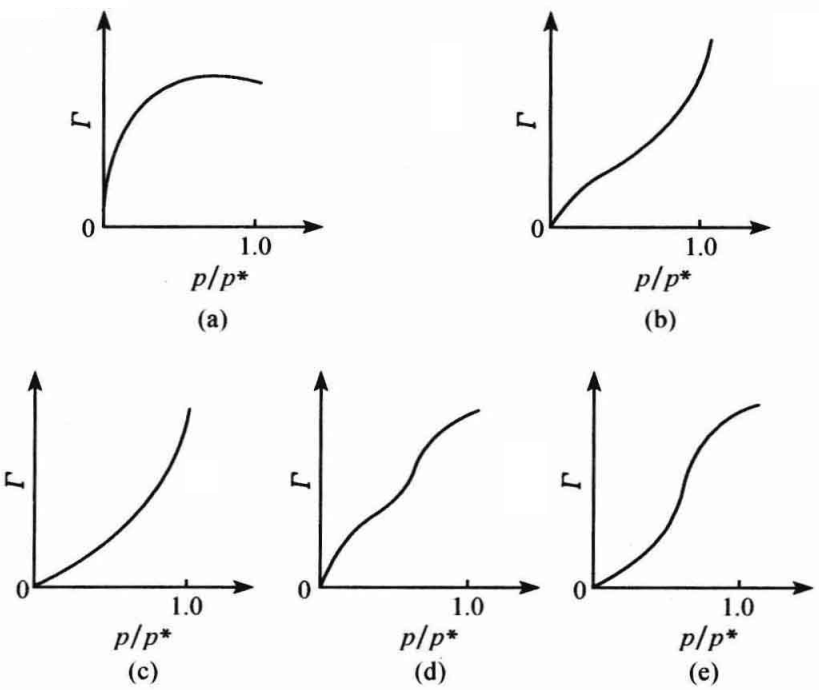
\includegraphics[width=.45\linewidth]{figures/fig8.15.png}
    \end{figure}

\end{frame}


\begin{frame}
    \frametitle{吸附理论}

    \begin{itemize}
        \item[1.] \cbf{弗兰德里希定温式}
    \end{itemize}
    根据实验结果，弗兰德里希（Freundlich）提出一个经验公式
    \[
        \varGamma = kp^{1/n} \qquad (n>1)
    \]
    取对数
    \[
        \lg \varGamma = \frac{1}{n} \lg p + \lg k
    \]
    以$\lg \varGamma$对$\lg p$作图得一直线，截距为$\lg k$，斜率为$\frac{1}{n}$。可求得k和n的值。

    弗兰德里希定温式在中等压力范围内能较好地适用于(a)类定温线，有一定的用途，但是它只是一个经验式，没有提供任何关于吸附机理的信息，只能代表一部分事实。

\end{frame}


\begin{frame}
    \frametitle{吸附理论}

    \begin{itemize}
        \item[2.] \cbf{朗缪尔定温式及单分子层吸附理论}
    \end{itemize}

    朗缪尔单分子层吸附理论的基本假设如下：
    \begin{enumerate}
        \item 催化剂表面各处的吸附能力是均匀的，各吸附位具有相同的能量        
        \item 吸附是单分子层的
        \item 被吸附分子间不发生相互作用，吸附分子的解吸概率不受邻近其他吸附分子的影响
        \item 吸附是一个可逆过程，气体在固体表面上的吸附是气体分子的吸附与解吸两种相反过程达到动态平衡的结果。
    \end{enumerate}
    定温下吸附平衡时，吸附速率等于解吸速率
    \[
        k_1p(1-\theta) = k_{-1}\theta
    \]

\end{frame}


\begin{frame}
    \frametitle{吸附理论}

    \begin{itemize}
        \item[2.] \cbf{朗缪尔定温式及单分子层吸附理论}
    \end{itemize}
    \[
        \theta=\frac{k_{1} p}{k_{-1}+k_{1} p} = \frac{\varGamma}{\varGamma_{\mathrm{m}}}
    \]
    令$b = \frac{k_1}{k_{-1}}$，则
    \[
        \varGamma=\varGamma_{\mathrm{m}} \theta=\varGamma_{\mathrm{m}} \frac{b p}{1+b p}
    \]
    \[
        \frac{p}{\varGamma}=\frac{1}{\varGamma_{\mathrm{m}} b}+\frac{p}{\varGamma_{\mathrm{m}}}
    \]
    上述式子均称为朗缪尔吸附定温式。$b$是吸附平衡常数，其大小代表了固体表面吸附气体能力的强弱。$\varGamma_{\mathrm{m}}$和$b$在一定温度下对一定吸附体系是常数。

    朗缪尔吸附定温式能很好地符合图(a)，可以较好地说明化学吸附。但是由于该理论假设固体表面均匀且只能形成单分子层，因此在实用中有一定的局限性。

\end{frame}


\begin{frame}
    \frametitle{吸附理论}

    \begin{itemize}
        \item[3.] \cbf{BET吸附定温式及多分子层吸附理论}
    \end{itemize}
    由于大多数固体对气体的吸附并不是单分子层吸附，尤其是物理吸附，往往是多分子层吸附，因此其吸附定温线不符合朗缪尔定温式。1938年，Brunauer、Emmett、Teller在朗缪尔理论的基础上，提出了多分子层吸附理论，并推导出著名的BET公式。

    多分子层吸附理论的其改进之处是假设：
    \begin{enumerate}
        \item 吸附是多分子层的
        \item 第一层是气体分子与固体表面分子直接作用引起的吸附，而第二层以后则是气体分子间相互作用产生的吸附。
        \item 在一定温度下，当吸附达到平衡时，气体的吸附量$\varGamma$等于各层吸附量的总和。
    \end{enumerate}

\end{frame}


\begin{frame}
    \frametitle{吸附理论}

    \begin{itemize}
        \item[3.] \cbf{BET吸附定温式及名分子层吸附理论}
    \end{itemize}
    经过比较复杂的数学运算，BET推出定温下吸附平衡时
    \[
        \varGamma=\frac{\varGamma_{\mathrm{m}} C p}{(p^{*}-p)\left[1+(C-1) \frac{p}{p^{*}}\right]}
    \]
    \begin{itemize}
        \item $\varGamma$为平衡压力$p$时的吸附量；
        \item $\varGamma_{\mathrm{m}}$为固体表面盖满单分子层时的吸附量；
        \item $p^*$为实验温度下气体的饱和蒸气压；
        \item $C$为与吸附热有关的常数，反映固体表面和气体分子间作用力的强弱程度
        \item BET吸附定温式也有一定的局限性，不能说明所有的吸附定温线。
    \end{itemize}

\end{frame}


\begin{frame}
    \frametitle{吸附与催化}

    吸附与催化是密切相关的。
    
    发现气-固相的多相催化作用是通过反应分子在催化剂表面上的吸附来实现的。反应分子首先吸附在固体表面的某些部位上，形成活化的表面中间化合物，使反应的活化能降低，反应加速，再经过脱附而得到产物。
        \begin{minipage}{0.68\linewidth}
            对于气-固相催化反应来说，固体表面是反应的场所，比表面的大小直接影响反应速率。因此多采用比表面大的海绵状或多孔性的催化剂。

            固体表面是不均匀的，在表面上有活性的地方只占催化剂表面的很少部分，只有当反应物被吸附到活性中心上才能形成化学键。

            催化剂的催化活性与化学吸附的强弱有密切的关系。
        \end{minipage}\hfill
        \begin{minipage}{0.28\linewidth}
            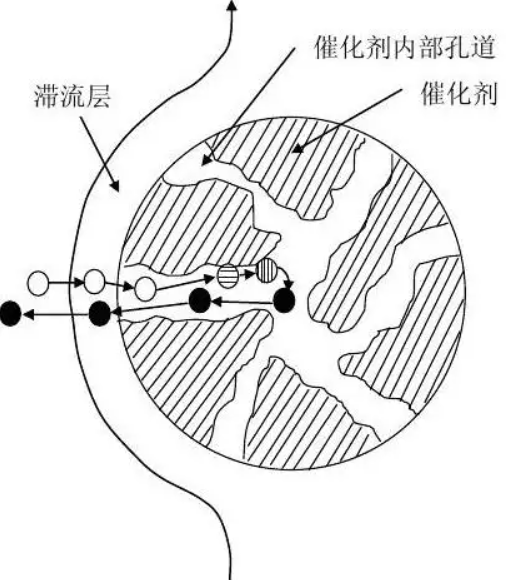
\includegraphics[width=\linewidth]{figures/catalyst.png}
        \end{minipage}
    

\end{frame}